\normaltrue \difficilefalse \tdifficilefalse
\correctionfalse

%\UPSTIidClasse{11} % 11 sup, 12 spé
%\newcommand{\UPSTIidClasse}{12}

\exer{Treuil de levage $\star$ \label{CIN:03:C2:06:91}}
\marginnote{\textit{Banque PT -- SIB 2023.}}
%\marginnote{%\UPSTIcompetence[2]{C2-06}}
\marginnote{\xpComp{CIN}{03}}%\UPSTIcompetence[2]{A3-05}}
\setcounter{question}{0}

\index{Compétence C2-06}\index{Compétence CIN-03}
%\index{Train d'engrenages simple}
\ifcorrection
\else
\marginnote{\textbf{Pas de corrigé pour cet exercice.}}
\fi

\ifprof
\else
On s’intéresse à un vérin électrique dont le schéma cinématique est donné ci-dessous. On donne $p$ le pas de la vis. On note $\eta_r$ le rendement d'un étage de réduction et $\eta_v$ le rendement de la vis.
\begin{marginfigure}
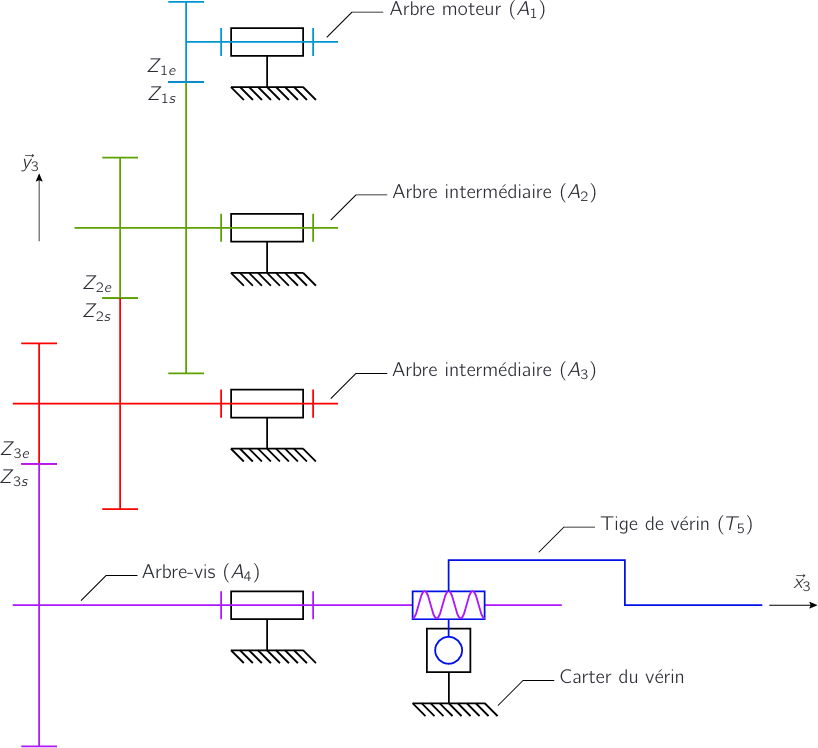
\includegraphics[width=\linewidth]{91_01}
\end{marginfigure}


\fi


\question{Donner le lien entre $\omega_v$ la vitesse de rotation de la vis et $V$ la vitesse de translation de la tige. }
\ifprof
\begin{corrige}
$V =\dfrac{p}{2\pi} \omega_v$
\end{corrige}
\else
\fi

\question{Donner l’expression de la vitesse $V$ en fonction de $\omega_m$.}
\ifprof 
\begin{corrige}
Dans un train simple, on a : $\dfrac{\omega_{v/0}}{\omega_{m/0}} = (-1)^n \dfrac{Z_{1e}Z_{2e}Z_{3e}}{Z_{1s}Z_{2s}Z_{3s}}$ avec $n=3$ nombre de contacts extérieurs.

Et donc $V(T_5/0) =-\dfrac{p}{2\pi} \dfrac{Z_{1e}Z_{2e}Z_{3e}}{Z_{1s}Z_{2s}Z_{3s}} \omega_{m/0}$.

\end{corrige}
\else

\fi





\ifprof
\else

\marginnote{Corrigé voir \ref{CIN:03:C2:06:91}.}

\fi